    \documentclass[10.5pt]{article}
    \usepackage{amsmath,amssymb,amsthm}
    \usepackage{listings}
    \usepackage{graphicx}
    \usepackage[shortlabels]{enumitem}
    \usepackage{tikz}
    \usepackage[margin=1in]{geometry}
    \usepackage{fancyhdr}
    \usepackage{epsfig} %% for loading postscript figures
    \usepackage{amsmath}
    \usepackage{float}
    \usepackage{amssymb}
    \usepackage{caption}
    \usepackage{subfigure}
    \usepackage{graphics}
    \usepackage{titlesec}
    \usepackage{mathrsfs}
    \usepackage{amsfonts}
    \usepackage{indentfirst}
    \usepackage{fontspec}
    \usepackage{xcolor}
    \renewcommand{\baselinestretch}{1.2}%Adjust Line Spacing
    %\geometry{left=2.0cm,right=2.0cm,top=2.0cm,bottom=2.0cm}% Adjust Margins of the File
    \usepackage{tikz-qtree}
    \usetikzlibrary{graphs}
    \tikzset{every tree node/.style={minimum width=2em,draw,circle},
    	blank/.style={draw=none},
    	edge from parent/.style=
    	{draw,edge from parent path={(\tikzparentnode) -- (\tikzchildnode)}},
    	level distance=1.2cm}
    \setlength{\parindent}{0pt}
    %\setlength{\parskip}{5pt plus 1pt}
    \setlength{\headheight}{13.6pt}
    \newcommand\question[2]{\vspace{.25in}\hrule\textbf{#1: #2}\vspace{.5em}\hrule\vspace{.10in}}
    \renewcommand\part[1]{\vspace{.10in}\textbf{(#1)}}
    \newcommand\algorithm{\vspace{.10in}\textbf{Algorithm: }}
    \newcommand\correctness{\vspace{.10in}\textbf{Correctness: }}
    \newcommand\runtime{\vspace{.10in}\textbf{Running time: }}
    \pagestyle{fancyplain}
    % Create horizontal rule command with an argument of height
    \newcommand{\horrule}[1]{\rule{\linewidth}{#1}}
    % Set the title here
    \title{
        \normalfont \normalsize
        \textsc{ShanghaiTech University} \\ [25pt]
        \horrule{0.5pt} \\[0.4cm] % Thin top horizontal rule
        \huge CS101 Algorithms and Data Structures\\ % The assignment title
        \LARGE Fall 2020\\
        \LARGE Homework 20\\
        \horrule{2pt} \\[0.5cm] % Thick bottom horizontal rule
    }
    % wrong usage of \author, never mind
    \author{}
    \date{Due date: 23:59, November 30, 2019}
    
    % set the header and footer
    \pagestyle{fancy}
    \lhead{CS101 Algorithms and Data Structures}
    \chead{Homework 6}
    \rhead{Due date: 23:59, October 26, 2019}
    \cfoot{\thepage}
    \renewcommand{\headrulewidth}{0.4pt}
    
    % special settings for the first page
    \fancypagestyle{firstpage}
    {
    	\renewcommand{\headrulewidth}{0pt}
    	\fancyhf{}
    	\fancyfoot[C]{\thepage}
    }
    
    % Add the support for auto numbering
    % use \problem{title} or \problem[number]{title} to add a new problem
    % also \subproblem is supported, just use it like \subsection
    \newcounter{ProblemCounter}
    \newcounter{oldvalue}
    \newcommand{\problem}[2][-1]{
    	\setcounter{oldvalue}{\value{secnumdepth}}
    	\setcounter{secnumdepth}{0}
    	\ifnum#1>-1
    		\setcounter{ProblemCounter}{0}
    	\else
    		\stepcounter{ProblemCounter}
    	\fi
    	\section{Problem \arabic{ProblemCounter}: #2}
    	\setcounter{secnumdepth}{\value{oldvalue}}
    }
    \newcommand{\subproblem}[1]{
    	\setcounter{oldvalue}{\value{section}}
    	\setcounter{section}{\value{ProblemCounter}}
    	\subsection{#1}
    	\setcounter{section}{\value{oldvalue}}
    }
    
    \setmonofont{Consolas}
    \definecolor{blve}{rgb}{0.3372549 , 0.61176471, 0.83921569}
    \definecolor{gr33n}{rgb}{0.29019608, 0.7372549 , 0.64705882}
    \makeatletter
    \lst@InstallKeywords k{class}{classstyle}\slshape{classstyle}{}ld
    \makeatother
    \lstset{language=C++,
            basicstyle=\ttfamily,
            keywordstyle=\color{blve}\ttfamily,
            stringstyle=\color{red}\ttfamily,
            commentstyle=\color{green}\ttfamily,
    		morecomment=[l][\color{magenta}]{\#},
    		classstyle = \bfseries\color{gr33n}, 
    		tabsize=4
    }
    
    
    \begin{document}
    
    \maketitle
    \thispagestyle{firstpage}
    %\newpage
    \vspace{3ex}
    
    \begin{enumerate}
    \item Please write your solutions in English. 
    
    \item Submit your solutions to gradescope.com.  
    
    \item Set your FULL Name to your Chinese name and your STUDENT ID correctly in Account Settings. 
    
    \item If you want to submit a handwritten version, scan it clearly. Camscanner is recommended. 
    
    \item When submitting, match your solutions to the according problem numbers correctly. 
    
    \item No late submission will be accepted.
    
    \item Violations to any of the above may result in zero grade. 
    \end{enumerate}
    \newpage
    

    %---------------------------------------------------------------
\problem{Multiple Choices}
Multiple Choices: Each question has one or more correct answer(s). Select all the correct answer(s). For each question, you get $0$ point if you select one or more wrong answers, but you get half points if you select a non-empty subset of the correct answers.\\
\textit{Note that you should write you answers of Problem 1 in the table below.}
\begin{table}[htbp]
	\begin{tabular}{|p{1.5cm}|p{1.5cm}|p{1.5cm}|}
	\hline 
	Q(1) & Q(2) & Q(3) \\
	\hline 
	\color{brown}&\color{brown}&\color{brown}\\ 
	\hline 
	\end{tabular} 
\end{table} \\
%%%%% (1)
(1) Topological Sort can be carried out on what kinds of graphs:
\begin{enumerate}[(A)]
	\item All weight acyclic graphs
	\item All directed graphs
	\item All (Directed) Trees
	\item All unweight directed acyclic graphs
	\item All cyclic directed graphs
\end{enumerate}
~\\
%%%%% (2)
(2) Which of the following statement about Dijkstra's algorithm is/are true?
\begin{enumerate}[(A)]
	\item Dijkstra's algorithm could only find the shortest path on directed graph.
	\item Dijkstra's algorithm could only find the shortest path on non-negative weighted graph.
	\item If we add a constraint that each node can only pass once, then Dijkstra's algorithm could find the shortest path on non-negative weighted graph.
	\item If we add a constraint that each edge can only pass once, then Dijkstra's algorithm could find the shortest path on non-negative weighted graph.
\end{enumerate}
~\\
%%%%% (3)
(3) Which of the following statement about Dijkstra's algorithm is/are true?
\begin{enumerate}[(A)]
	\item  Dijkstra's algorithm with a binary heap could run in time $ \Theta ((|V|+|E|)\log |V|)$.
	\item  Dijkstra's algorithm on a tree with a binary heap could run in time $ {\Theta (|E|+|V|)}$.
	\item Dijkstra's algorithm on connected graphs with a binary heap could run in time $ \Theta (|E|\log |V|)$.
	\item None of above.
\end{enumerate}
\newpage
% -------------------------------------------------------------------------
\problem{Dijkstra's algorithm}
Given a weighted graph below, please run Dijkstra's algorithm using vertex $A$ as the source. Write down the vertices in the order which they are marked and the updated distances at each step. Please use $\infty$ to represent initial value.
	
	\begin{figure}[htbp]
		\centering
		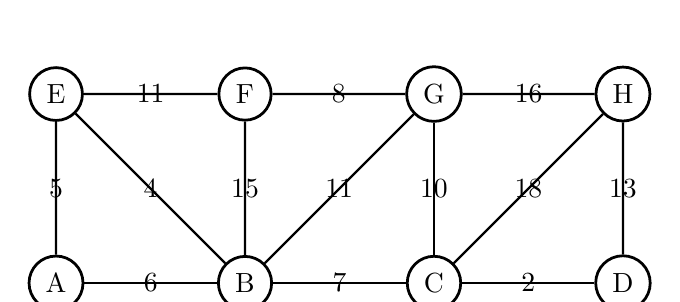
\begin{tikzpicture}
		[thick,scale=0.8, every node/.style={scale=1}]
		%		\node[circle] (n0){A};
		\node[circle, draw, line width=1pt] (a) at (-4.5,0){A};
		\node[circle, draw, line width=1pt] (b) at (-1.5,0){B};
		\node[circle, draw, line width=1pt] (c) at (1.5,0){C};
		\node[circle, draw, line width=1pt] (d) at (4.5,0){D};
		\node[circle, draw, line width=1pt] (e) at (-4.5,3){E};
		\node[circle, draw, line width=1pt] (f) at (-1.5,3){F};
		\node[circle, draw, line width=1pt] (g) at (1.5,3){G};
		\node[circle, draw, line width=1pt] (h) at (4.5,3){H};
		\draw[-] (a) to node{6} (b);
		\draw[-] (a) to node{5} (e);
		\draw[-] (b) to node{7} (c);
		\draw[-] (b) to node{4} (e);
		\draw[-] (b) to node{15} (f);
		\draw[-] (b) to node{11} (g);
		\draw[-] (c) to node{2} (d);
		\draw[-] (c) to node{10} (g);
		\draw[-] (c) to node{18} (h);
		\draw[-] (d) to node{13} (h);
		\draw[-] (e) to node{11} (f);
		\draw[-] (f) to node{8} (g);
		\draw[-] (g) to node{16} (h);
		\end{tikzpicture}
	\end{figure}
	\vspace{-10pt}
	\textbf{Solution}:
	\vspace{-15pt}
	\begin{table}[htbp]
		\begin{center}  
			\begin{tabular}{|l|l| p{3cm}|}  
				\hline  
				step & vertex\\ \hline  
				1 &   \\ \hline    
				2 &   \\ \hline    
				3 &   \\ \hline    
				4 &   \\ \hline    
				5 &   \\ \hline   
				6 &   \\ \hline    
				7 &   \\ \hline   
				8 &   \\  
				\hline  
			\end{tabular}  
		\end{center}  
	\end{table}
	\vspace{-25pt}
	\begin{table}[htbp]
		\begin{center}  
			\begin{tabular}{|l|l|l|l|l|l|l|l|l| p{3cm}|}  
				\hline  
				step & dist[A] & dist[B] & dist[C] & dist[D] & dist[E] & dist[F] & dist[G] & dist[H]\\ \hline  
				1 &   &   &   &   &   &   &   &  \\ \hline    
				2 &   &   &   &   &   &   &   &  \\ \hline    
				3 &   &   &   &   &   &   &   &  \\ \hline    
				4 &   &   &   &   &   &   &   &  \\ \hline    
				5 &   &   &   &   &   &   &   &  \\ \hline   
				6 &   &   &   &   &   &   &   &  \\ \hline    
				7 &   &   &   &   &   &   &   &  \\ \hline   
				8 &   &   &   &   &   &   &   &  \\  
				\hline  
			\end{tabular}  
		\end{center}  
	\end{table}
\pagebreak

%------------------------------------------------------------------
\problem{Providing Counterexample}
For the following three statements, please provide counterexamples to illustrate that these three statements are pseudo-proposition.
	\begin{enumerate}[(a)]
		\item A directed graph with |V| vertices and |V|-1 edges has a unique Topological sort result.
		\vspace{64pt}
		\item If G is a connected and undirected graph without negative cycles, we can apply Dijkstra's algorithm to find the shortest path.
		\vspace{64pt}
		\item Assume that we use the priority queue to implement Dijkstra's algorithm on a non-negative graph, then we can do the following operation. When the terminate vertex is pushed into the priority queue, we can stop the algorithm so that we can get the shortest path without running the algorithm until popping the terminate vertex from the priority queue
		\vspace{64pt}
		
	\end{enumerate}

\pagebreak

%------------------------------------------------------------------
\problem{Topological sort counting}

		\begin{center}
	
		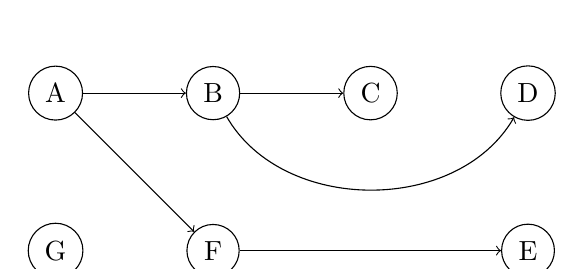
\begin{tikzpicture}
			\node[shape=circle,draw=black] (A) at (0,0) {A};
			\node[shape=circle,draw=black] (B) at (2,0) {B};
			\node[shape=circle,draw=black] (C) at (4,0) {C};
			\node[shape=circle,draw=black] (D) at (6,0) {D};
			\node[shape=circle,draw=black] (E) at (6,-2) {E};
			\node[shape=circle,draw=black] (F) at (2,-2) {F};
			\node[shape=circle,draw=black] (G) at (0,-2) {G};
		
			\path [->](A) edge node {} (B);
			\path [->](B) edge[] node {} (C);
			\path [->](B) edge[bend right=60] node {} (D);
			\path [->](F) edge[] node {} (E);
			\path [->](A) edge[] node {} (F); 
		\end{tikzpicture}
	\end{center}
	\begin{enumerate}[(a)]
		\item Show a topological sort result.
		\vspace{64pt}
		\item Count the number of different topological sort result (show your process).
		\vspace{64pt}
		
	\end{enumerate}
\pagebreak
%-----------------------------------------------------------------

\end{document}
